% !TEX TS-program = pdflatex
% !TEX encoding = UTF-8 Unicode

% This is a simple template for a LaTeX document using the "article" class.
% See "book", "report", "letter" for other types of document.

\documentclass[11pt]{article} % use larger type; default would be 10pt

\usepackage[utf8]{inputenc} % set input encoding (not needed with XeLaTeX)

%%% Examples of Article customizations
% These packages are optional, depending whether you want the features they provide.
% See the LaTeX Companion or other references for full information.

%%% PAGE DIMENSIONS
\usepackage{geometry} % to change the page dimensions
\geometry{a4paper} % or letterpaper (US) or a5paper or....
% \geometry{margin=2in} % for example, change the margins to 2 inches all round
% \geometry{landscape} % set up the page for landscape
%   read geometry.pdf for detailed page layout information

\usepackage{graphicx} % support the \includegraphics command and options

% \usepackage[parfill]{parskip} % Activate to begin paragraphs with an empty line rather than an indent

%%% PACKAGES
\usepackage{booktabs} % for much better looking tables
\usepackage{array} % for better arrays (eg matrices) in maths
%\usepackage{paralist} % very flexible & customisable lists (eg. enumerate/itemize, etc.)
\usepackage{verbatim} % adds environment for commenting out blocks of text & for better verbatim
\usepackage{subfig} % make it possible to include more than one captioned figure/table in a single float
% These packages are all incorporated in the memoir class to one degree or another...

%%% HEADERS & FOOTERS
\usepackage{fancyhdr} % This should be set AFTER setting up the page geometry
\pagestyle{fancy} % options: empty , plain , fancy
\renewcommand{\headrulewidth}{0pt} % customise the layout...
\lhead{}\chead{}\rhead{}
\lfoot{}\cfoot{\thepage}\rfoot{}

%%% SECTION TITLE APPEARANCE
\usepackage{sectsty}
\allsectionsfont{\sffamily\mdseries\upshape} % (See the fntguide.pdf for font help)
% (This matches ConTeXt defaults)

%%% ToC (table of contents) APPEARANCE
\usepackage[nottoc,notlof,notlot]{tocbibind} % Put the bibliography in the ToC
\usepackage[titles,subfigure]{tocloft} % Alter the style of the Table of Contents
\renewcommand{\cftsecfont}{\rmfamily\mdseries\upshape}
\renewcommand{\cftsecpagefont}{\rmfamily\mdseries\upshape} % No bold!

%%% END Article customizations

\usepackage[spanish]{babel}
\usepackage{listings} 
%%% The "real" document content comes below...

\title{Investigación de Lenguajes - LIP}
\author{Rodrigo Castro\\Jorge Vergara\\Oswaldo Bayona}
%\date{} % Activate to display a given date or no date (if empty),
         % otherwise the current date is printed 

\begin{document}
\maketitle
%\tableofcontents % No hace falta un TOC en un artículo corto

\section{Introducción}

\section{Características}


\section{Historia}


\section{Tutorial de Instalación}
Un interprete que podemos utilizar para programar en Lisp es DrRacket. Su instalacion es muy sencilla y rapida.
El entorno de trabajo para programar en este lenguaje se puede apreciar en la Figura 5


\begin{figure}[h]
\centering
    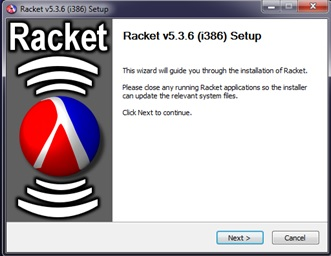
\includegraphics{imagenes_investigacion/paso_uno.jpg}
\caption {}
\label{Figura 1}
\end{figure}

\begin{figure}[h]
\centering
    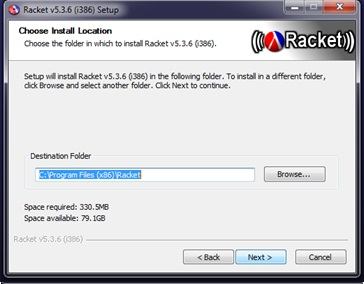
\includegraphics{imagenes_investigacion/paso_dos.jpg}
\caption { }
\label{Figura 2}
\end{figure}

\begin{figure}[h]
\centering
    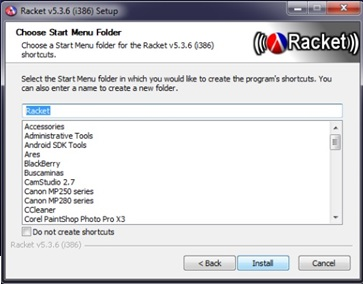
\includegraphics{imagenes_investigacion/paso_tres.jpg}
\caption { }
\label{Figura 3}
\end{figure}

\begin{figure}[h]
\centering
    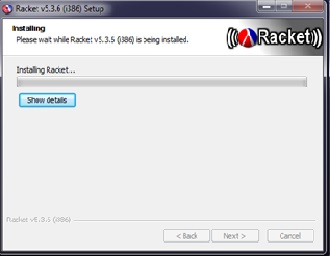
\includegraphics{imagenes_investigacion/paso_cuatro.jpg}
\caption { }
\label{Figura 4}
\end{figure}


\begin{figure}[h]
\centering
    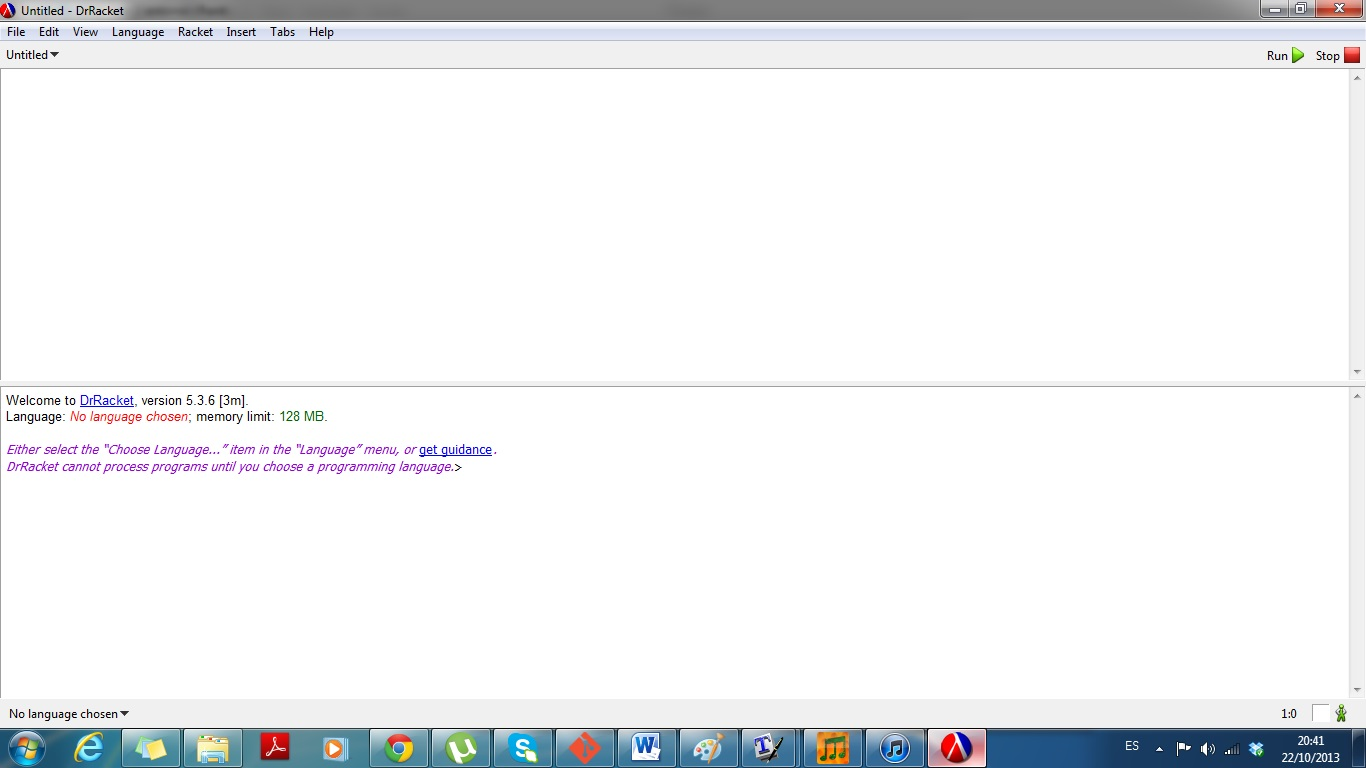
\includegraphics[width=450pts] {imagenes_investigacion/entorno.jpg}
\caption {//Entorno de trabajo de DrRocket}
\label{Figura 5}
\end{figure}



\section{Hola Mundo y otros Programas Introductorios}


%hola mundo
\subsection{Hola Mundo}
\lstset{language=LISP}          

%codigo
\begin{lstlisting}[frame=single] 
	(defun HolaMundo()
		(print 'Hola Mundo')]

\end{lstlisting}

\subsection{Factorial}

% calcular suma de una lista
\lstset{language=LISP}          % Set your language (you can change the language for each code-block optionally)

%codigo 
\begin{lstlisting}[frame=single]
	
	;Calculo del factorial de un numero
	(defun Factorial(n)
		(cond( ( lessp n 2) 1)
			(t  (* n  (Factorial(sub 1 n))] 
\end{lstlisting}

Como se puede ver la funcion factorial tiene una estructura recursiva, adiferencia de los lenguajes de pogramacion tradificionales que tienen sentencias especializadas para realizar iteraciones en LIP no contamos con esas herramientas.\\
Descripcion de la funcion:
1.- como paso base vemos si el numero ingresado es menor que 2 en este caso devolvemos 1
2.-si el numero no es menor que 2 este numero lo multipilcamos por el factorial de n-1 

\subsection{Calcular Media Aritmetica de una Lista}

Para resolver este problema lo vamos a dividir en 3 funciones mas bacisas
\\  \\
La primera funcion que vamos a desarrolar es "Suma" que calcula la sumatoria de cada elemento de la lista
% calcular suma de una lista
\lstset{language=LISP}          % Set your language (you can change the language for each code-block optionally)

%codigo 
\begin{lstlisting}[frame=single]
	
	;Suma todos los elementos de una lista
	(defun Suma(lista)
		(cond((null lista) 0 )
			((atom lista) lista)
			(t  (+ (car lista) (suma (cdr lista))] 
\end{lstlisting}

Detallando un poco la funcion:\\
1.- en el caso que la lista este vacia nuestra funcion devuelve 0 nuestro primer caso base\\
2.- si nuestra lista es un atomo es decir un simple numero devolvemos la lista este seria otro caso base\\
3.- en el caso que la lista aun tenga mas de 1 elemento tomamos el 1 elemento de la lista y lo sumamos al resto de elementos de la lista\\

Como segunda parte desarrolarremos una funcion que cuente la cantidad de elementos que se encuentran en la lista

% contar elementos de la lista
\lstset{language=LISP}          % Set your language (you can change the language for each code-block optionally)

%codigo 
\begin{lstlisting}[frame=single]
	
	;cuenta los elementos de la lista
	(defun Contar(lista)
		(cond((null lista) 0 )
			((atom lista) 1)
			(t (addl (contar (cdr lista)] 
\end{lstlisting}






\end{document}